\chapter{Discussione in merito al lavoro svolto}

\begin{preamble}
{\em
Il prossimo capitolo sarà incentrato sull'analisi del lavoro dedicato alla creazione dell'applicazione Android. In particolare, saranno esaminate le differenze e le similitudini con l'applicazione Vivino, attualmente molto popolare tra gli utenti, al fine di mettere in evidenza le potenzialità dell'applicazione mobile oggetto della tesi. \newline \indent Successivamente, verrà condotta un'approfondita analisi SWOT dei rischi associati allo sviluppo e alla futura distribuzione dell'applicazione.
}
\end{preamble}

\section{Confronto con l'app Vivino}

Vivino è una popolare app mobile e una piattaforma online che si concentra sulla degustazione e sulla condivisione di recensioni e informazioni sul vino. Gli utenti di Vivino possono utilizzare l'app per scansionare etichette di bottiglie di vino e ottenerne informazioni dettagliate, come recensioni, punteggi, descrizioni, abbinamenti cibo-vino e prezzi. Inoltre, gli utenti possono anche recensire i vini, tenere traccia dei loro preferiti e connettersi con altri amanti del vino sulla piattaforma.

Vivino è diventato uno strumento popolare per gli appassionati di vino che desiderano esplorare e scoprire nuovi prodotti, condividere le proprie esperienze e prendere decisioni informate sugli acquisti. La piattaforma contiene una vasta quantità di dati sul vino e offre una comunità di appassionati del settore in cui è possibile condividere opinioni e consigli.

Il progetto condivide molti aspetti in comune con l'applicazione Vivino, poiché entrambi sfruttano il riconoscimento delle bottiglie di vino attraverso l'utilizzo della fotocamera. Tuttavia, le differenze risiedono negli obiettivi in quanto Vivino si concentra sulla creazione di una community di appassionati del vino che condividono recensioni e descrizioni sui prodotti vitivinicoli. D'altra parte, l'applicazione oggetto della tesi combina le informazioni di base sul vino con lo stato di salute del vigneto di provenienza, utilizzando sia i dati satellitari che i dati provenienti dalla stazione IoT.

\begin{figure}[h]
	\centering
	
\includegraphics [width=.45\columnwidth, angle=0]
            {logoVivino}
	\caption{Logo dell'applicazione Vivino}
	\label{7fig:logoVivino}
\end{figure}

\section{SWOT Analysis del progetto}

L'analisi SWOT (\textit{Strengths}, \textit{Weaknesses}, \textit{Opportunities}, \textit{Threats}) è uno strumento di pianificazione e valutazione dei rischi utilizzato nelle aziende, nelle organizzazioni, e nella pianificazione personale. Consiste nell'identificazione e nell'analisi dei punti di forza, delle debolezze, delle opportunità e delle minacce rilevanti in una determinata situazione o contesto. I fattori chiave dell'analisi SWOT sono:

\begin{itemize}

	\item Punti di forza \textit{(Strengths)}: identifica i punti di forza interni che possono mitigare i rischi.
	
	\item Debolezze \textit{(Weaknesses)}: identifica le debolezze interne che possono aumentare i rischi.

	\item Opportunità \textit{(Opportunities)}: identifica le opportunità esterne che possono ridurre i rischi o fornire alternative.
	
	\item Minacce \textit{(Threats)}: identifica le minacce esterne che possono aumentare i rischi.

\end{itemize}

Per condurre una \textit{SWOT analysis}, è importante identificare con precisione questi fattori, sia interni che esterni. Gli elementi interni sono sotto il controllo dell'organizzazione e possono essere influenzati direttamente, mentre gli elementi esterni sono fuori dal controllo dell'organizzazione ma possono comunque avere un impatto significativo sulla sua strategia.

Una \textit{SWOT analysis} aiuta da identificare come sfruttare i punti di forza e le opportunità, mitigare i punti deboli e affrontare le minacce. Questa analisi fornisce una base solida per la pianificazione strategica e la presa di decisioni aziendali informate.

Per condurre la \textit{SWOT Analysis} dei rischi, è importante definire il concetto di \textit{Smoke Test}. Lo \textit{Smoke Test}rappresenta una metodologia essenziale per la validazione di un'idea di business, garantendo che il prodotto o servizio proposto sia realmente in linea con le aspettative dei futuri clienti.

Lo scopo principale di questo test è determinare se i potenziali clienti manifestano un interesse reale per l'offerta. La chiave del successo è far percepire loro che il prodotto o servizio è già disponibile sul mercato. Questo processo è cruciale per validare l'idea e coinvolgere potenziali clienti ancor prima del lancio ufficiale del prodotto.

Nel prossimo capitolo dedicato agli sviluppi futuri, l'argomento verrà approfondito nel dettaglio indicando delle possibili strategie per l'esecuzione dello Smoke Test dell'applicazione mobile.

Di seguito, per ogni rischio individuato nello sviluppo e messa in produzione dell'applicazione, ne verrà mostrata la relativa  \textit{SWOT Analysis}. 

\subsection{Difficoltà nella diffusione dell'applicazione tra gli utenti}

Si può prevedere il rischio che l'applicazione incontri delle difficoltà nella sua diffusione tra gli utenti in quanto esiste una forte competizione con delle applicazioni mobile già presenti sul mercato da molti anni. L'analisi SWOT di questo rischio è riportata in Figura \ref{7fig:tabellaDiffusioneUtenti}.

\begin{figure}[h]
	\centering
	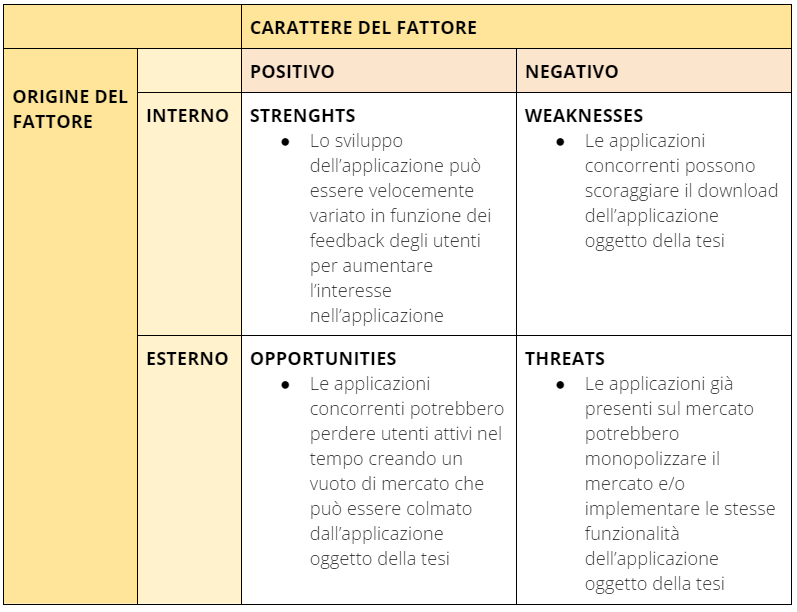
\includegraphics [width=.99\columnwidth, angle=0]
            {tabellaDiffusioneUtenti}
	\caption{SWOT Analysis del rischio associato alla difficoltà nella diffusione dell'applicazione tra gli utenti}
	\label{7fig:tabellaDiffusioneUtenti}
\end{figure}

\subsection{Difficoltà nello sviluppo futuro dell'applicazione}

Si può prevedere il rischio che l'applicazione incontri delle difficoltà durante il suo sviluppo software. Il progetto è in continua evoluzione e può portare lo sviluppo software verso sfide nuove ed impegnative che, per quanto stimolanti, espongono l'azienda a dei rischi notevoli. L'analisi SWOT di quest'ultimi è riportato in Figura \ref{7fig:tabellaSviluppoApplicazione}.

\begin{figure}[h]
	\centering
	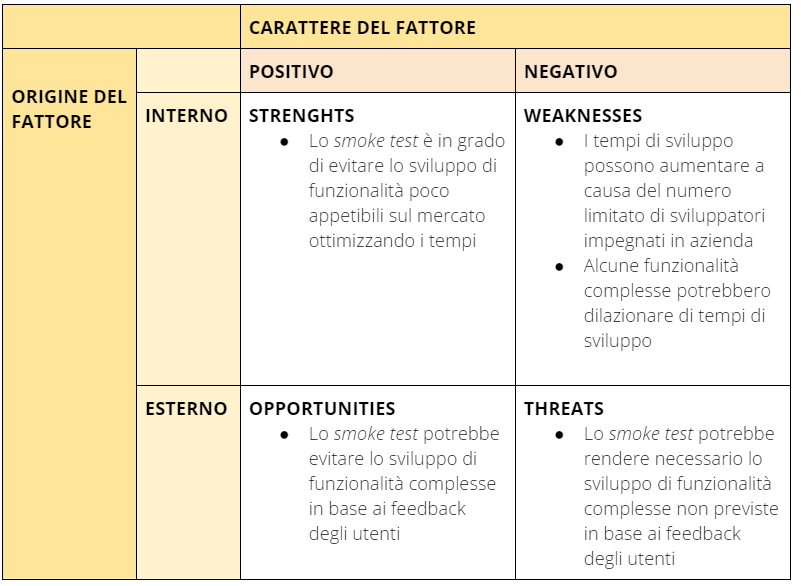
\includegraphics [width=.99\columnwidth, angle=0]
            {tabellaSviluppoApplicazione}
	\caption{SWOT Analysis del rischio associato alla difficoltà nello sviluppo futuro dell'applicazione}
	\label{7fig:tabellaSviluppoApplicazione}
\end{figure}

\subsection{Difficoltà nella presentazione dei dati nell'applicazione}

Si può prevedere il rischio che l'applicazione mostri troppe informazioni all'utente, scoraggiandone l'utilizzo e riducendone il tempo di permanenza. L'analisi SWOT di questo rischio è riportata in Figura \ref{7fig:tabellaPresentazioneDati}.

\begin{figure}[t]
	\centering
	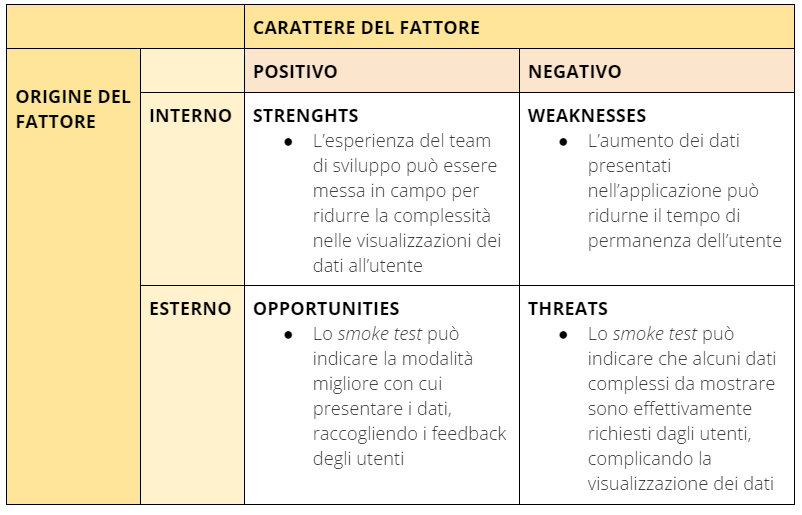
\includegraphics [width=.99\columnwidth, angle=0]
            {tabellaPresentazioneDati}
	\caption{SWOT Analysis del rischio associato alla presentazione dei dati nell'applicazione}
	\label{7fig:tabellaPresentazioneDati}
\end{figure}
